\begin{minipage}{0.75\linewidth}
\begin{figure}[h]
    \centering
    \begin{adjustbox}{max width=1.0\linewidth, keepaspectratio}
        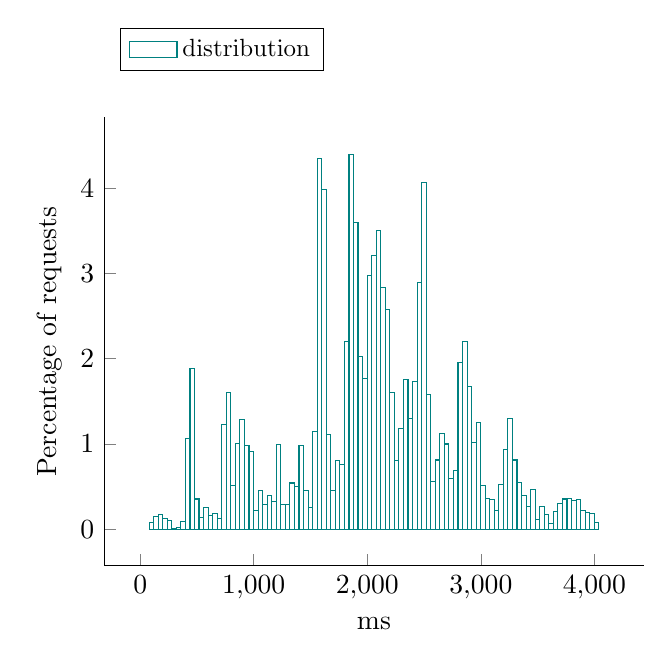
\begin{tikzpicture}
            \begin{axis}[ylabel = Percentage of requests, 
xlabel = ms, 
legend style = {nodes={scale=0.9, transform shape}, at={(0.03,1.2)}, anchor=north west, draw=black, fill=white, align=left, legend columns=3},
area style, mark size = 0pt,
 cycle list name = exotic,
  axis lines* = left]
		\addplot +[ybar interval] coordinates {
			 (78, 0.0833073)
			 (118.01, 0.145788)
			 (158.02, 0.177028)
			 (198.03, 0.124961)
			 (238.04, 0.104134)
			 (278.05, 0.0104134)
			 (318.06, 0.0208268)
			 (358.07, 0.0937207)
			 (398.08, 1.06217)
			 (438.09, 1.88483)
			 (478.1, 0.354056)
			 (518.11, 0.135374)
			 (558.12, 0.249922)
			 (598.13, 0.156201)
			 (638.14, 0.187441)
			 (678.15, 0.124961)
			 (718.16, 1.22878)
			 (758.17, 1.60367)
			 (798.18, 0.510257)
			 (838.19, 1.0101)
			 (878.2, 1.29126)
			 (918.21, 0.978861)
			 (958.22, 0.91638)
			 (998.23, 0.218682)
			 (1038.24, 0.45819)
			 (1078.25, 0.291576)
			 (1118.26, 0.39571)
			 (1158.27, 0.322816)
			 (1198.28, 0.989274)
			 (1238.29, 0.291576)
			 (1278.3, 0.291576)
			 (1318.31, 0.541497)
			 (1358.32, 0.499844)
			 (1398.33, 0.978861)
			 (1438.34, 0.45819)
			 (1478.35, 0.249922)
			 (1518.36, 1.14548)
			 (1558.37, 4.35281)
			 (1598.38, 3.98834)
			 (1638.39, 1.11424)
			 (1678.4, 0.45819)
			 (1718.41, 0.801833)
			 (1758.42, 0.760179)
			 (1798.43, 2.20764)
			 (1838.44, 4.39446)
			 (1878.45, 3.60304)
			 (1918.46, 2.03062)
			 (1958.47, 1.77028)
			 (1998.48, 2.97824)
			 (2038.49, 3.20733)
			 (2078.5, 3.50932)
			 (2118.51, 2.83245)
			 (2158.52, 2.58253)
			 (2198.53, 1.60367)
			 (2238.54, 0.801833)
			 (2278.55, 1.17672)
			 (2318.56, 1.75987)
			 (2358.57, 1.30168)
			 (2398.58, 1.72863)
			 (2438.59, 2.89493)
			 (2478.6, 4.07164)
			 (2518.61, 1.58284)
			 (2558.62, 0.562324)
			 (2598.63, 0.812246)
			 (2638.64, 1.12465)
			 (2678.65, 0.999688)
			 (2718.66, 0.593565)
			 (2758.67, 0.687285)
			 (2798.68, 1.95772)
			 (2838.69, 2.19723)
			 (2878.7, 1.67656)
			 (2918.71, 1.02051)
			 (2958.72, 1.24961)
			 (2998.73, 0.510257)
			 (3038.74, 0.364469)
			 (3078.75, 0.343643)
			 (3118.76, 0.218682)
			 (3158.77, 0.520671)
			 (3198.78, 0.937207)
			 (3238.79, 1.30168)
			 (3278.8, 0.812246)
			 (3318.81, 0.551911)
			 (3358.82, 0.39571)
			 (3398.83, 0.270749)
			 (3438.84, 0.468604)
			 (3478.85, 0.114548)
			 (3518.86, 0.270749)
			 (3558.87, 0.177028)
			 (3598.88, 0.0624805)
			 (3638.89, 0.208268)
			 (3678.9, 0.301989)
			 (3718.91, 0.354056)
			 (3758.92, 0.364469)
			 (3798.93, 0.333229)
			 (3838.94, 0.343643)
			 (3878.95, 0.218682)
			 (3918.96, 0.197855)
			 (3958.97, 0.187441)
			 (3998.98, 0.0833073)
			 (4038.99, 0.0833073)
		};
\addlegendentry{distribution};
           \end{axis}
      \end{tikzpicture}
  \end{adjustbox}
  \caption{Response time distribution - req = ReadUser-0}
\end{figure}
\end{minipage}\hfill\begin{minipage}{0.18\linewidth}
\begin{table}[h]
\begin{tabular}{|cc|}
\hline
\textbf{} & \textbf{ms}\\ \hline
 \Xhline{0.005\arrayrulewidth}
min & 78\\
 \Xhline{0.005\arrayrulewidth}
max & 4079\\
 \Xhline{0.005\arrayrulewidth}
mean & 2060\\
 \Xhline{0.005\arrayrulewidth}
std & 772\\
\hline
\hline
 \Xhline{0.005\arrayrulewidth}
25th & 1606\\
 \Xhline{0.005\arrayrulewidth}
50th & 2066\\
 \Xhline{0.005\arrayrulewidth}
75th & 2512\\
 \Xhline{0.005\arrayrulewidth}
80th & 2694\\
 \Xhline{0.005\arrayrulewidth}
85th & 2861\\
 \Xhline{0.005\arrayrulewidth}
90th & 3000\\
 \Xhline{0.005\arrayrulewidth}
95th & 3319\\
 \Xhline{0.005\arrayrulewidth}
99th & 3851\\
\hline
\end{tabular}
\caption{Response time}
\end{table}
\end{minipage}\hfill